

\documentclass{beamer}
\usetheme{default}
\usepackage{hyperref,url,german}
\usepackage{graphicx} % Allows including images
\usepackage{booktabs} % Allows the use of \toprule, \midrule and 
\setbeamertemplate{caption}{\raggedright\insertcaption\par}
\colorlet{shadecolor}{gray!90}

%----------------------------------------------------------------------------------------
%	TITLE PAGE
%----------------------------------------------------------------------------------------

\title{H"aufige Missverst"andnisse "uber den p-Wert}

\author{Dr. med. Andreas Mock, MSc, MPhil} % Your name
\institute{Nationales Centrum f"ur Tumorerkrankungen (NCT) Heidelberg}
\date{28.11.2017} % Date, can be changed to a custom date
\titlegraphic{
\includegraphics[width=5cm]{../Intro_to_R/nct_logo}}

\begin{document}

%----------------------------------------------------------------------------------------
%	PRESENTATION SLIDES
%---------------------------------------------------------------------------------------
\begin{frame}
	\maketitle
\end{frame}

\begin{frame}
	\frametitle{Der Erfinder des p-Werts}
\begin{figure}
	\begin{columns}
			\column{.5\textwidth}
			\centering
			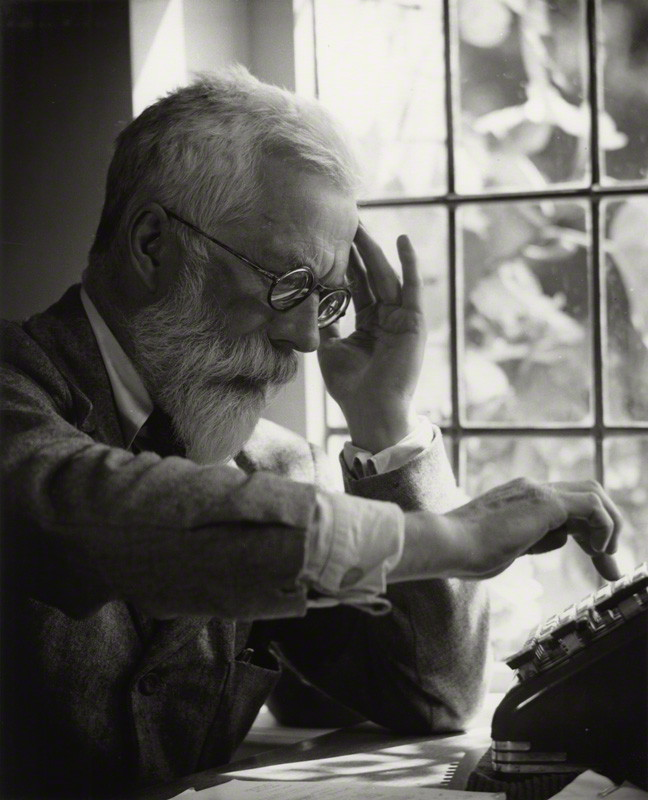
\includegraphics[width=1\linewidth]{Fisher}
			\caption{\textbf{Sir Ronald Fisher (1890-1962)} Gonville \& Caius College, Cambridge}
			\label{fig:Fisher}
	\column{.5\textwidth}
		\textit{\glqq Personally, the writer prefers to set a low standard of significance at the 5 percent point $[...]$ A scientific fact should be regarded as experimentally established only if a properly designed experiment rarely fails to give this level of significance.\grqq}\\
		\vspace{1em}
		 {\footnotesize Statistical Methods for Research Workers, 1926}
	\end{columns}
\end{figure}	
\end{frame}

\begin{frame}
	\frametitle{Definition des p-Wertes}
	Wahrscheinlichkeit das gleiche Stichprobenergebnis oder ein noch extremeres zu erhalten, wenn die Nullhypothese wahr ist.\\
	\vspace{1em}
	 Algebraische Definition: P(X \geq x \mid~ $H_0$) wobei $X$ eine Zufallsvariable und $x$ der beobachte Wert in den Daten ist 
\begin{figure}
\centering
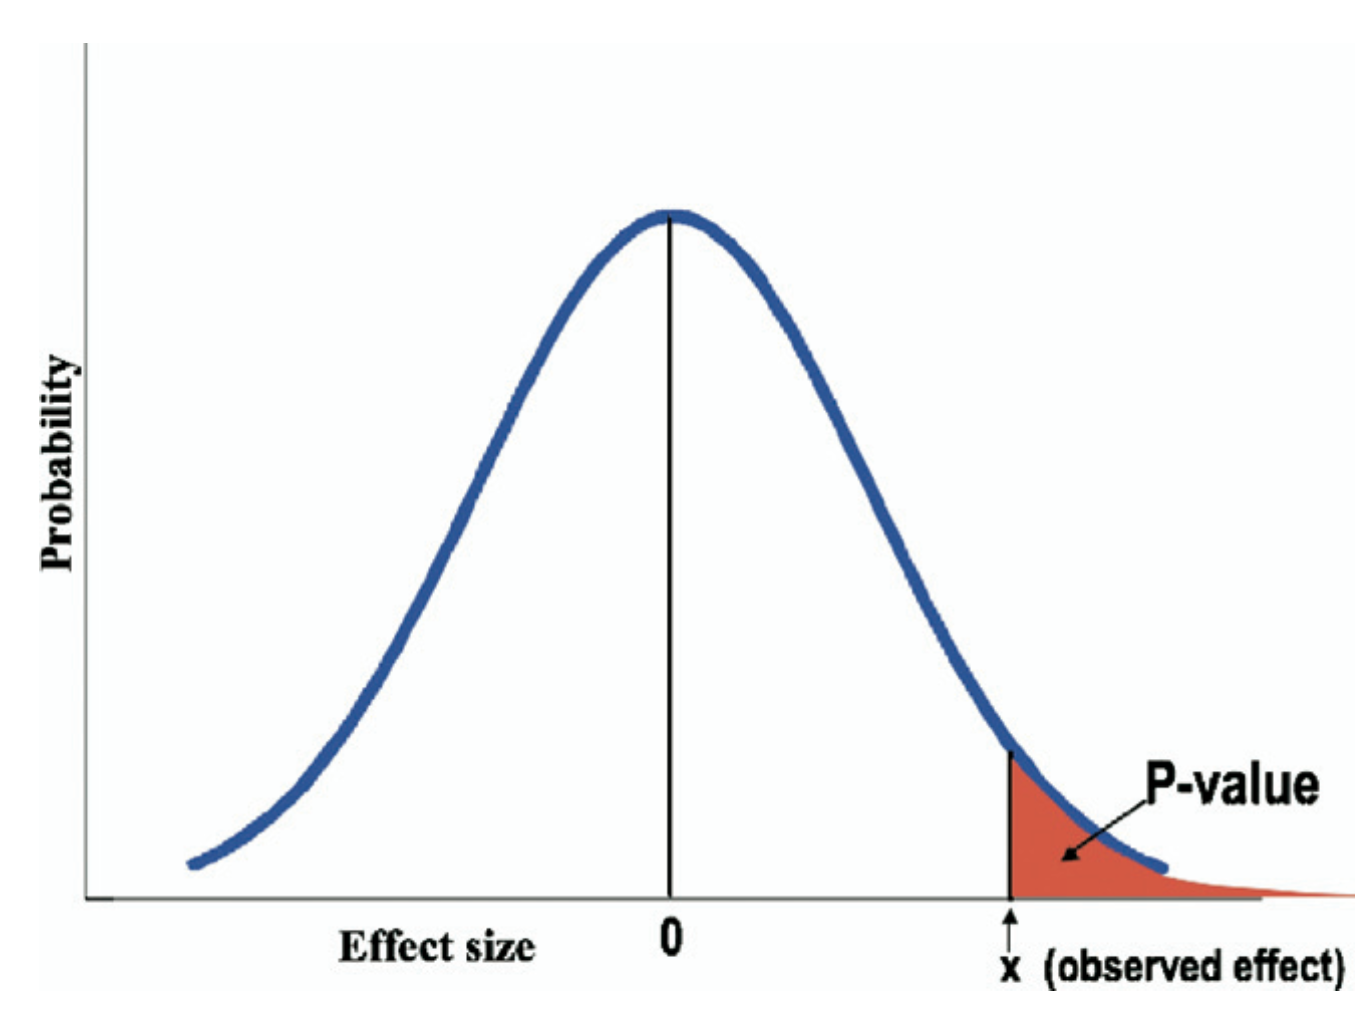
\includegraphics[width=0.5\linewidth]{bell_curve}
\caption{{\footnotesize Goodman, 2008}}
\label{fig:bell_curve}
\end{figure}
\end{frame}

\begin{frame}
	\frametitle{\#1 $\mid$ Wenn p\textless0.05, ist die Nullhypothese nur in 5\% wahr}
	Dies ist die wohl \textbf{h"aufigste Fehlinterpretation} des p-Wertes. \\
	\vspace{1em}
	Der p-Wert wird unter der Annahme berechnet, dass die Nullhypothese zutrifft (P(Daten \mid~$H_0$)), er kann daher nicht gleichzeitig die Wahrscheinlichkeit sein, dass die Nullhypothese zutrifft (P($H_0$ \mid Daten)).\\
	\vspace{1em}
	\textbf{Beispiel}: Die Wahrscheinlichkeit drei Mal hinter einander Kopf beim M"unzwurf zu erhalten ist p=0.125. Dies bedeutet jedoch nicht, dass die Wahrscheinlichkeit, dass die M"unze fair ist nur 12.5\% betr"agt.	
\end{frame}

\begin{frame}
	\frametitle{\#2 $\mid$ p\textgreater 0.05 bedeutet, dass es keinen Unterschied zwischen den Gruppen gibt}
	Eine nicht signifikante Differenz bedeutet blo\ss{}, dass die beobachten \textbf{Daten konsistent mit der Nullhypothese} sind und nicht, dass die Nullhypothese wahrscheinlicher ist.
\end{frame}

\begin{frame}
	\frametitle{\#3 $\mid$ p=0.06 ist substantiell schlechter als p=0.04}
	Fisher hat den p-Wert als \textbf{kontinuierliche Variable} eingef"uhrt um abzusch"atzen, ob ein Ergebnis es Wert ist weiter untersucht zu werden. Die magische p-Wert Grenze von 0.05 ist \textbf{v"ollig arbitr"ar}. p-Werte von 0.04 und 0.06 sind sehr "ahnliche Wahrscheinlichkeiten!
	\begin{figure}
		\centering
		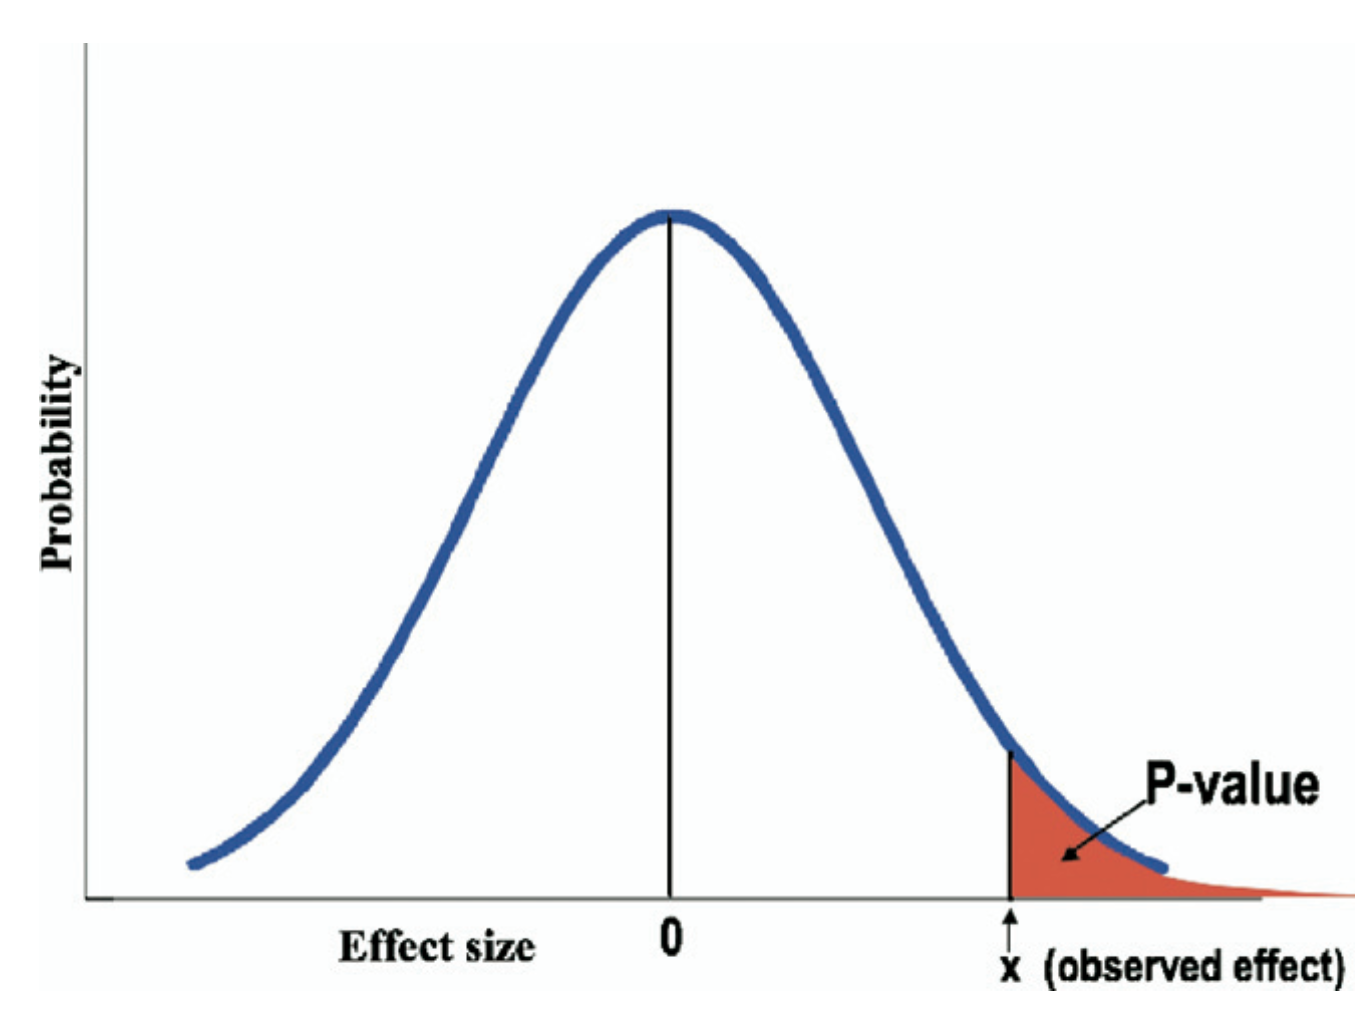
\includegraphics[width=0.5\linewidth]{bell_curve}
		\caption{{\footnotesize Goodman, 2008}}
		\label{fig:bell_curve}
	\end{figure}
\end{frame}

\begin{frame}
	\frametitle{\#4 $\mid$ Studien mit gleichem p-Wert zeigen eine "ahnlich starke Effektgr"osse}
	
	Der folgende Plot zeigt, dass dies nicht zutrifft. Der gleiche p-Wert kann einen v"ollig anderen Effekt indizieren (Fig. B). Umgekehrt, kann es einen identischen Effekt bei unterschiedlichem p-Wert geben (Fig. A):
\begin{figure}
\centering
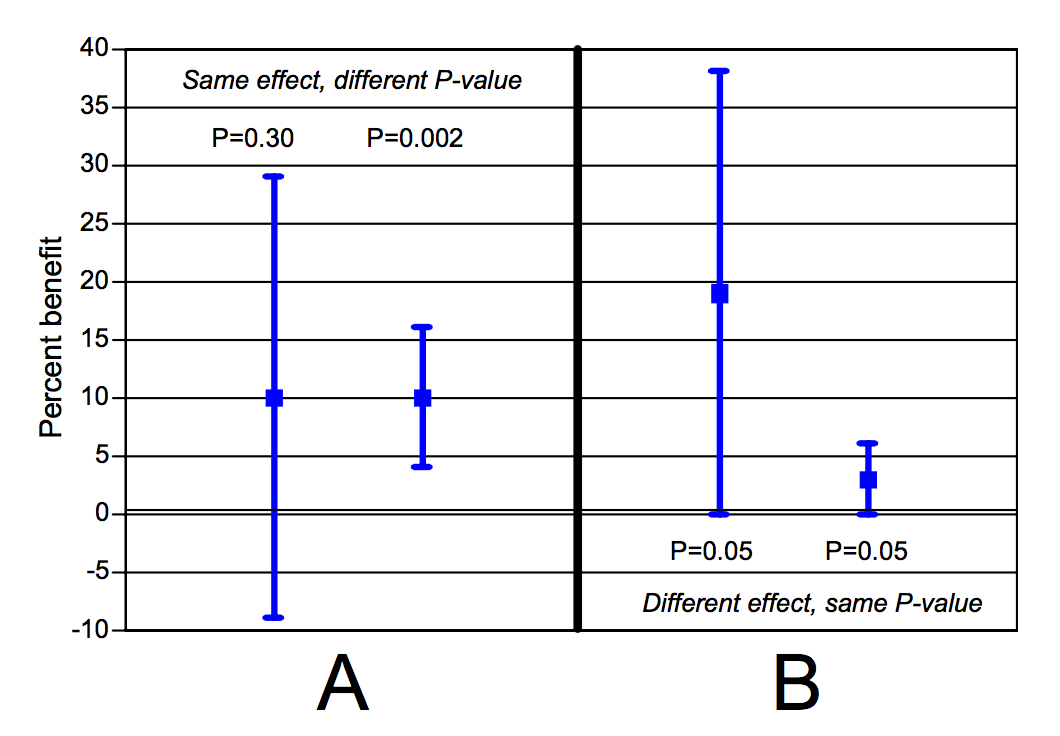
\includegraphics[width=0.65\linewidth]{effect}
\caption{{\footnotesize Goodman, 2008}}
\label{fig:effect}
\end{figure}
\end{frame}

\begin{frame}
	\frametitle{\#5 $\mid$ p=0.05 bedeutet, dass man bei Wiederholung des Experiments in 5\% ein nicht signifikantes Ergebnis erh"alt }
	
\begin{columns}
		
\column{0.35\textwidth}

\begin{figure}
\centering
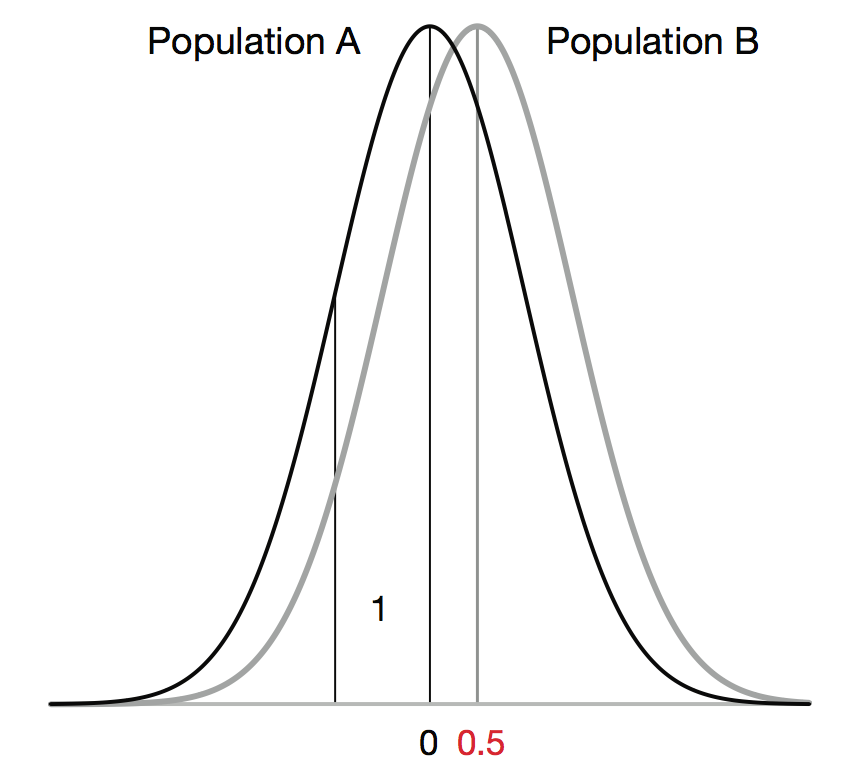
\includegraphics[width=1.2\linewidth]{simulated_populations}
\label{fig:simulated_populations}
\end{figure}

\column{0.65\textwidth}
	
\begin{figure}
\centering
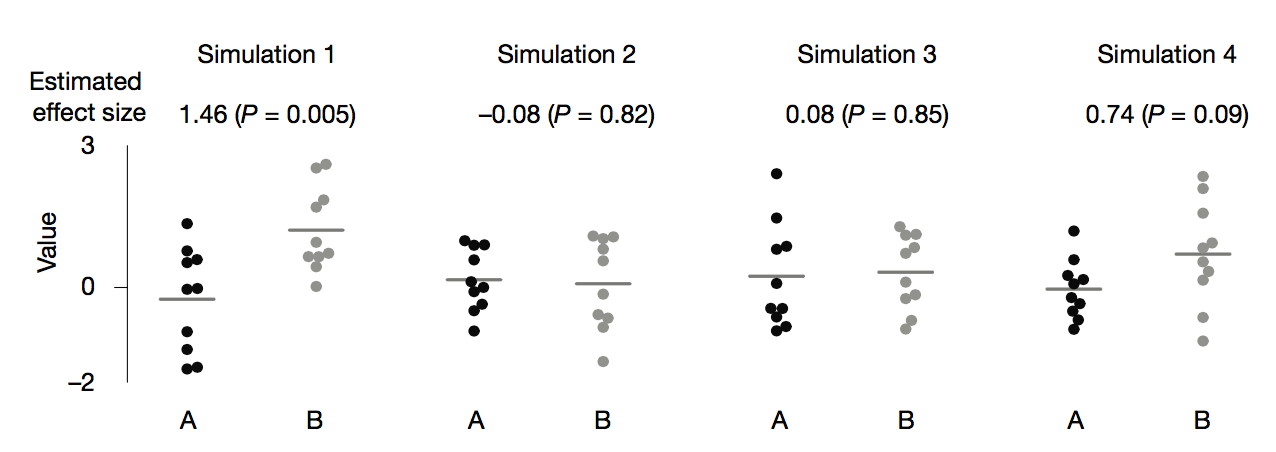
\includegraphics[width=1\linewidth]{simulations}
\caption{{\footnotesize Halsey et al., 2015}}
\label{fig:simulations}
\end{figure}
\end{columns}
\vspace{2em}
Nur bei	einer \textbf{gro\ss{}en Effektgr"osse bzw. Power} \\
(i.e. Gruppengr"o\ss{}e) sind p-Werte bei Wiederholung des Experiments mit einer anderen Stichprobe reproduzierbar!
\end{frame}

\begin{frame}
	\frametitle{Literatur}
	\begin{itemize}
		\item \textbf{A Dirty Dozen: Twelve P-Value Misconceptions}\\
		Goodman, S\\
		Semin Hematol. 2008 Jul;45(3):135-40.
		\vspace{1em}
			\item \textbf{The fickle P value generates irreproducible results}\\
			Halsey LG, Curran-Everett D, Vowler SL \& Drummond GB\\
			Nat Methods. 2015 Mar;12(3):179-85. 
	\end{itemize}
\end{frame}

\end{document}